% (The MIT License)
%
% Copyright (c) 2023-2024 Yegor Bugayenko
%
% Permission is hereby granted, free of charge, to any person obtaining a copy
% of this software and associated documentation files (the 'Software'), to deal
% in the Software without restriction, including without limitation the rights
% to use, copy, modify, merge, publish, distribute, sublicense, and/or sell
% copies of the Software, and to permit persons to whom the Software is
% furnished to do so, subject to the following conditions:
%
% The above copyright notice and this permission notice shall be included in all
% copies or substantial portions of the Software.
%
% THE SOFTWARE IS PROVIDED 'AS IS', WITHOUT WARRANTY OF ANY KIND, EXPRESS OR
% IMPLIED, INCLUDING BUT NOT LIMITED TO THE WARRANTIES OF MERCHANTABILITY,
% FITNESS FOR A PARTICULAR PURPOSE AND NONINFRINGEMENT. IN NO EVENT SHALL THE
% AUTHORS OR COPYRIGHT HOLDERS BE LIABLE FOR ANY CLAIM, DAMAGES OR OTHER
% LIABILITY, WHETHER IN AN ACTION OF CONTRACT, TORT OR OTHERWISE, ARISING FROM,
% OUT OF OR IN CONNECTION WITH THE SOFTWARE OR THE USE OR OTHER DEALINGS IN THE
% SOFTWARE.

\documentclass{article}
\usepackage{../painofoop}
\newcommand*\thetitle{Getters}
\newcommand*\thesubtitle{Accessors, Encapsulation, Printers}
\begin{document}

\plush{\poopTitlePage{3}{2YyVmIQQ23w}}

\pptToc

\plush{\pptChapter[Definition]{What is a Getter?}}

\qte
  {joshua-bloch}
  {If a class is accessible outside the confines of its package, the prudent programmer will provide \ul{accessor methods} to preserve the flexibility to change the class's internal representation.}
  {bloch2008effective}

\plush{
  \begin{multicols}{2}
  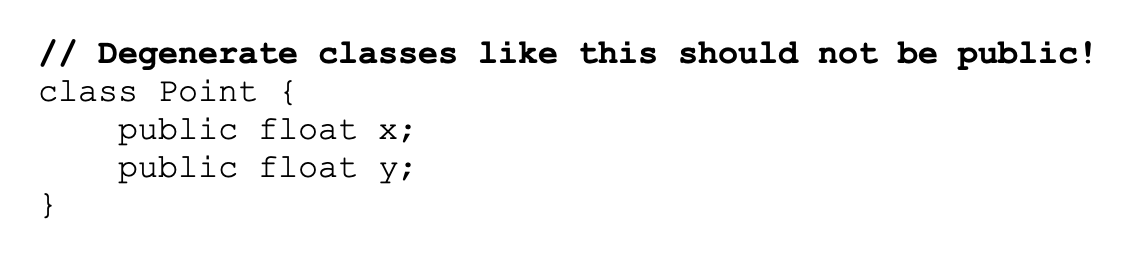
\includegraphics[width=.9\linewidth]{bloch-struct.png}
  \par
  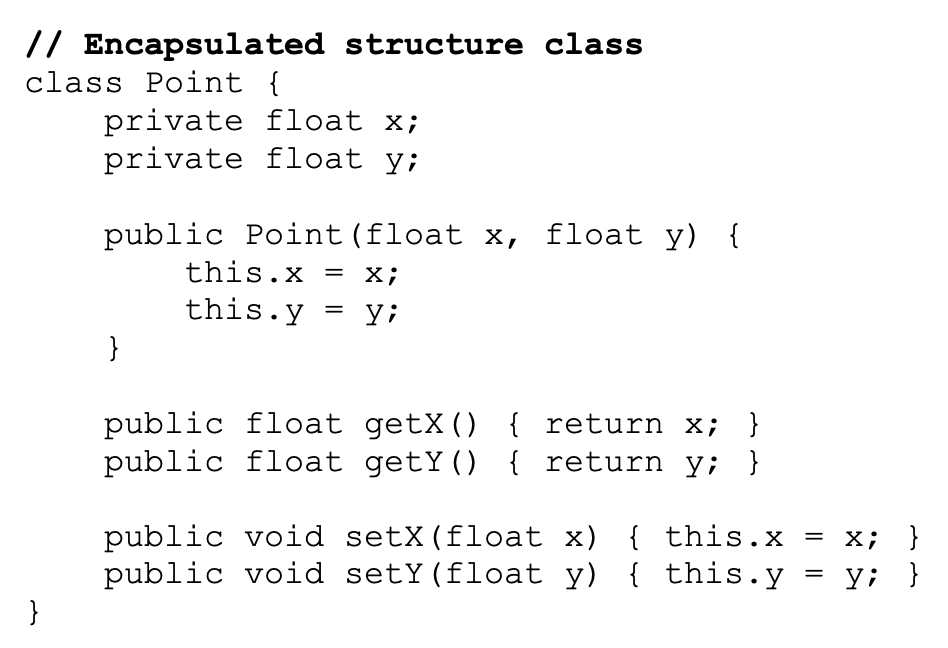
\includegraphics[width=.9\linewidth]{bloch-class.png}
  \par\columnbreak\par
  ``Because such classes are accessed by their data fields, they do not offer the benefits of \ul{encapsulation}. You cannot change the representation of such a class without changing its API, enforce any invariants, and take any auxiliary action when a field is modified. [...] such classes are \ul{anathema} and should always be replaced by classes with private fields and public \textcolor{orange}{accessor methods}.''
  \source{bloch2008effective}
  \end{multicols}}


\pptSection[What?]{Which one is a getter?}
\begin{pptWide}{2}
{\small\begin{ffcode}
class MiddleSquare {
  private short seed;
  MiddleSquare(short s) { seed = s; }

  (*@\textcolor{orange}{short getNextNumber()}@*) {
    int s = (int) seed * seed;
    seed = (short) (s >> 8);
    return seed;
  }
}
\end{ffcode}
}
\par\columnbreak\par
{\small\begin{ffcode}
class MiddleSquare {
  private short seed;
  MiddleSquare(short s) { seed = s; }

  (*@\textcolor{orange}{short getSeed()}@*) {
    return this.seed;
  }
}
\end{ffcode}
}
\end{pptWide}
\par
\plush{}

\pptSection[Boilerplate]{Boilerplate getters}
\begin{pptWide}{2}
{\small\begin{ffcode}
class Document
  def initialize(n)
    @name = n
  end
  (*@\textcolor{orange}{def name}@*)
    (*@\textcolor{orange}{@name}@*)
  (*@\textcolor{orange}{end}@*)
end
d = Document.new("/tmp/test.txt")
puts d.name
\end{ffcode}
}
\par\columnbreak\par
{\small\begin{ffcode}
class Document
  (*@\textcolor{orange}{attr\_reader}@*) :name
  def initialize(n)
    @name = n
  end
end

d = Document.new("/tmp/test.txt")
puts d.name
\end{ffcode}
}
\end{pptWide}
\par
Some modern programming languages (e.g. Ruby) offer an ability to generate the \ul{boilerplate} for mutators and accessors in a single line.
\plush{}

\pptSection[Purpose]{What getters are for?}
\begin{pptWide}{2}
\pptPic{0.8}{gpt-1.png}
\par\columnbreak\par
\pptPic{0.8}{gpt-2.png}
\end{pptWide}
\par
This is what GPT-4 replied to my question: ``Why should we use getters in Java instead of making class fields public? What are the benefits?''
\plush{}

\pptSection[DTO]{Data Transfer Objects (DTO)}
\begin{pptWide}{2}
{\small\begin{ffcode}
class BookDTO {
  private int id;
  private String author;
  private String title;
  BookDTO(int i, String a, String t)
    { id = i; author = a; title = t; }
  int getId() { return id; }
  String getAuthor() { return author; }
  String getTitle() { return title; }
}
\end{ffcode}
}
\par\columnbreak\par
{\small\begin{ffcode}
class JsonApi {
  BookDTO getById(int id) { /* ... */ }
}

BookDTO dto = api.getById(42);

print(dto(*@\textcolor{orange}{.getTitle()}@*));
print(dto(*@\textcolor{orange}{.getAuthor()}@*));
\end{ffcode}
}
\end{pptWide}
\par
There is no excuse for the use of DTO~\citep{bugayenko2016blog0706}. Almost...
\plush{}

\plush{\pptChapter{Encapsulation}}

\qte
  {../faces/grady-booch}
  {Encapsulation is most often achieved through \ul{information hiding}, which is the process of hiding all the \ul{secrets} of an object that do not contribute to its essential characteristics; typically, the structure of an object is hidden, as well as the implementation of its methods... Encapsulation provides \ul{explicit barriers} among different abstractions and thus leads to a clear separation of concerns.}
  {booch1994object}

\qte
  {../faces/david-west}
  {In most ways, encapsulation is a \ul{discipline} more than a real barrier; seldom is the \ul{integrity} of an object protected in any absolute sense, and this is especially true of software objects, so it is up to the user of an object to \ul{respect} that object's encapsulation.}
  {west2004object}

\pptSection[Integrity]{Who is protecting the integrity better?}
\begin{pptWide}{2}
{\small\begin{ffcode}
class User {
  private String name;
  User(String n) { name = n; }
  int getName() {
    return this.name;
  }
}
if (employees.contains(user(*@\textcolor{orange}{.getName()}@*))) {
  /* pay a salary */
}
\end{ffcode}
}
\par\columnbreak\par
{\small\begin{ffcode}
class User {
  private String name;
  User(String n) { name = n; }
  bool isEmployee() {
    return employees.contains(this.name);
  }
}
if (user(*@\textcolor{orange}{.isEmployee()}@*)) {
  /* pay a salary */
}
\end{ffcode}
}
\end{pptWide}
\par
Which class \ul{hides} its data better?
\plush{}

\pptSection[Semantic]{Who knows about data semantic?}
\begin{pptWide}{2}
{\small\begin{ffcode}
class Box {
  private int weight;
  Box(int kg) { weight = kg; }
  int getWeight() {
    return this.weight;
  }
}
int w = box(*@\textcolor{orange}{.getWeight()}@*);
int lbs = w / 0.454;
printf("The weight is \%d lbs\n");
\end{ffcode}
}
\par\columnbreak\par
{\small\begin{ffcode}
class Box {
  private int weight;
  Box(int kg) { weight = kg; }
  int getLbs() {
    return this.weight / 0.454;
  }
}
int lbs = box(*@\textcolor{orange}{.getLbs()}@*);
printf("The weight is \%d lbs\n");
\end{ffcode}
}
\end{pptWide}
\par
What happens if the \ff{Box} decides to store the \ff{weight} in pounds instead of kilograms? How will it know how many of its clients still assume that the \ff{weight} is in kilograms?~\citep{bugayenko2014blog0916}
\plush{}

\plush{\pptChapter[Alternative]{The Alternative}}

\qte
  {../faces/martin-fowler}
  {\textbf{Tell-Don't-Ask} principle: Rather than asking an object for data and acting on that data, we should instead \ul{tell} an object what to do. This encourages to move behavior into an object to go with the data.}
  {fowler2013tell}

\plush{
  \begin{multicols}{2}
  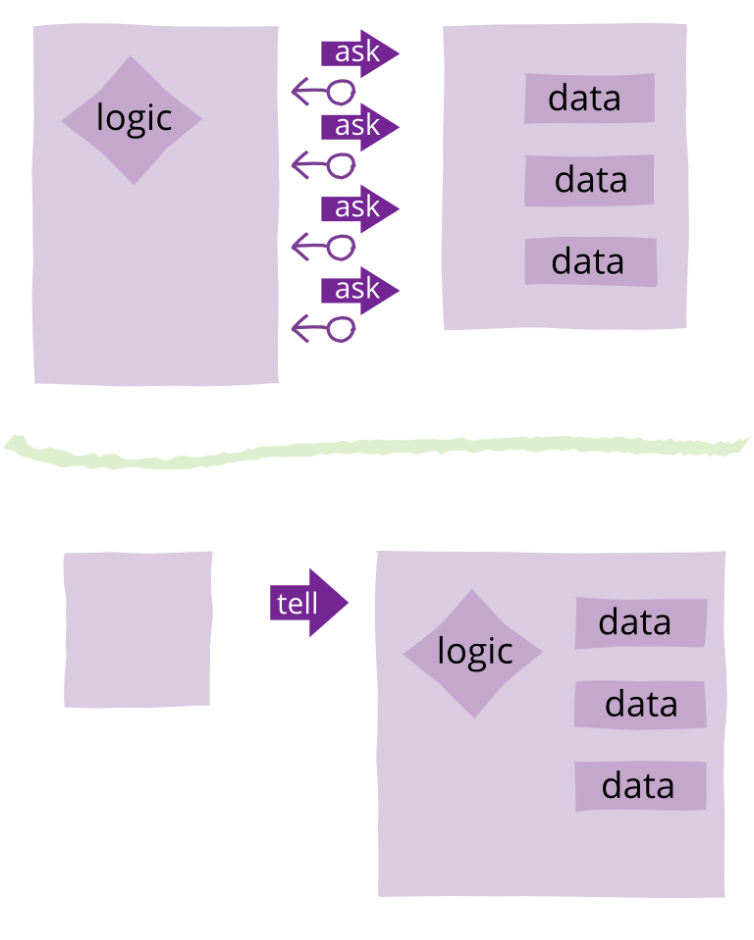
\includegraphics[width=.9\linewidth]{fowler-dontask.png}
  \par\columnbreak\par
  ``One of the fundamental principles of object-oriented design is to combine data and behavior, so that the basic elements of our system (objects) combine both together. This is often a good thing because this data and the behavior that manipulates them are \ul{tightly coupled}.''
  \source{fowler2013tell}
  \end{multicols}}

\pptSection[TellDontAsk]{1) Tell Don't Ask, an Example}
\begin{pptWide}{2}
{\small\begin{ffcode}
class BookDTO {
  private int id;
  private String author;
  private String title;
  BookDTO(int i, String a, String t)
    { id = i; author = a; title = t; }
  void print() { /* ... */ }
}
\end{ffcode}
}
\par\columnbreak\par
{\small\begin{ffcode}
class JsonApi {
  BookDTO getById(int id) { /* ... */ }
}

BookDTO dto = api.getById(42);
dto.print();
\end{ffcode}
}
\end{pptWide}
\par
The \ff{print()} method may also be called a ``printer''~\citep{bugayenko2016blog0405}.
\plush{}

\qte
  {../faces/allen-holub}
  {Though getter/setter methods are commonplace in Java, they are not particularly object-oriented. In fact, they can \ul{damage} your code's maintainability. Moreover, the presence of numerous getter and setter methods is a red flag that the program isn't necessarily well designed from an OO perspective.}
  {holub2003why}

\pptSection[NoPrefix]{2) Get rid of the ``get'' prefix}
\begin{pptWide}{2}
{\small\begin{ffcode}
class Book {
  private int id;
  private String author;
  private String title;
  Book(int i, String a, String t)
    { id = i; author = a; title = t; }
  int id() { return id; }
  String author() { return author; }
  String title() { return title; }
}
\end{ffcode}
}
\par\columnbreak\par
{\small\begin{ffcode}
class JsonApi {
  Book getById(int id) { /* ... */ }
}

Book book = api.getById(42);

print(book.author());
print(book.title());
\end{ffcode}
}
\end{pptWide}
\par
\plush{}

\pptSection[Public]{3) Make fields public}
\begin{pptWide}{2}
{\small\begin{ffcode}
class Book {
  public final int id;
  public final String author;
  public final String title;
  Book(int i, String a, String t)
    { id = i; author = a; title = t; }
}
\end{ffcode}
}
\par\columnbreak\par
{\small\begin{ffcode}
class JsonApi {
  Book getById(int id) { /* ... */ }
}

Book book = api.getById(42);

print(book.author);
print(book.title);
\end{ffcode}
}
\end{pptWide}
\par
\plush{}

\end{document}
